\chapter{Improved Parallel Composition}

\label{chap:ParComp}

The contents of this chapter is based on the results published previously in \cite{improved_par_comp}. The chapter covers in detail the proposed modification to the labelled Petri nets parallel composition algorithm allowing for simpler resulting nets while preserving result equivalence up to bisimulation.

\section{Improved parallel composition}\label{se-main}

The improved parallel composition algorithm extends the
conventional one by adding a pre-processing step, where some
places are removed from the components, as they are guaranteed
to be implicit in the result. To identify these places, one can
note that a place is required in the final composition only if
under some reachable marking it can be the place that
disables some transition in its postset.

For simplicity, consider the parallel composition
$C=C_1\parallel C_2$, whose components synchronise on a single
signal $s$ which is an output of $C_1$ and an input of $C_2$.
Let $(M_1,M_2)$ be a reachable marking of $C$, where $M_1$ and
$M_2$ are some reachable markings of $C_1$ and $C_2$,
respectively. Furthermore, suppose that $M_1$ enables, say,
$s^+$ in $C_1$, where $s$ is an output. Now, if $M_2$ does not
enable $s^+$ in $C_2$, where $s$ is an input, then there is
computation interference. Therefore, if the FCI assumption
holds, $M_2$ has to enable $s^+$ in $C_2$, \ie whenever $s^+$
is enabled in $C_1$, it is also enabled in $C_2$. In other
words, the firing of $s^+$ in $C$ is fully controlled by $C_1$,
and so \emph{the constraints on firing of $s$ that are present
in $C_2$ can be ignored}. This means that the places in the
preset of an $s^+$-labelled transition in $C_2$ will be
implicit in the composition (subject to some technical
conditions formulated below), and so can be removed before the
composition is performed.

The above is true for the simple case of STGs with injective
labelling and no dummies. However, the general picture is more
complicated. In case of non-injective labelling, there can be
multiple transitions corresponding to the same input signal
transition, and the FCI assumption only guarantees the
enabledness of one of them. Hence, some `memory' (in the form
of places) is required to trace which of these transitions has
to be fired, which prohibits the removal of places from their
presets. Furthermore, if the STG contains dummies, removing
places from their postsets introduces some undesirable effects
explained later. These considerations lead to the following
conditions of applicability of the proposed optimisation.

\begin{proposition}\label{pr-main}
Let $C\DEF\parallel_{i\in I}C_{i}$ be a composition of STGs
that satisfies the FCI property and yields an
output-determinate STG, and, for each $i\in I$, $C_{i}'$ be the
STG obtained from $C_{i}$ by deleting all places $p$ such that:
\begin{enumerate}[1.]
\item each transition $t\in\post{p}$ is labelled with a
    signal, say $s$, and:
\begin{enumerate}[a)]
\item\label{only-inputs-in-postset} $s$ is an input;
\item\label{exists-matching-output} there is an STG $C_j$ for which $s$ is an output;
\item\label{injective-labelling} there are at most one
    $s^+$- and at most one $s^-$-la\-bel\-led
    transition in $C_i$;
\end{enumerate}
\item\label{no-dummies-in-preset} $\pre{p}$ does not
    contain dummy transitions.
\end{enumerate}
Then $C'\DEF\parallel_{i\in I}C_i'$ and $C$ are bisimilar.
\end{proposition}

\begin{figure}[!tb]
  \centering
    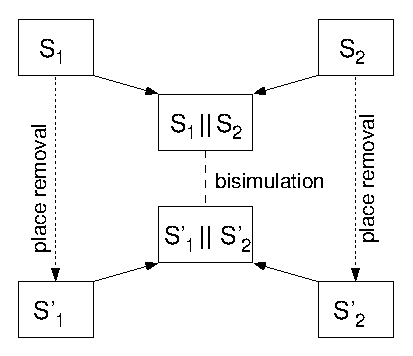
\includegraphics[scale=1]{fig/parallel_composition}
  \caption[Equivalence preservation by improved parallel composition]{\label{fi-parcomp-improvement-theorem}
    Equivalence preserved by place removal in improved parallel composition.
  }
\end{figure}

The proposition can be depicted schematically by a diagram in Fig.~\ref{fi-parcomp-improvement-theorem}.
Here the boxes named $S_1$ and $S_2$ represent the original STGs, 
$S_1'$ and $S_2'$ are represent STGs obtained from $S_1$ and $S_2$ by removing places according to
 the rules detailed above, and $S_1 \parallel S_2$ and $S_1' \parallel S_2'$ represent 
$S_1$ composed with $S_2$ and $S_1'$ composed with $S_2'$ respectively. 
We use a dashed line to signify the bisimulation relation between $S_1 \parallel S_2$ and $S_1' \parallel S_2'$.

 
The conditions~\ref{only-inputs-in-postset}
and~\ref{exists-matching-output} are intrinsic to the proposed
method, and essentially state that due to the FCI assumption,
firing of an input signal in a component can be controlled from
the outside (\viz by the component controlling the
corresponding output --- whose existence is ensured
by~\ref{exists-matching-output}), and so the component itself
can get rid of the places controlling it.

The conditions~\ref{injective-labelling}
and~\ref{no-dummies-in-preset} are technical restrictions on
application of our method. If
condition~\ref{injective-labelling} is violated, there are
several transitions that have the same label, say $s^+$ (where
$s$ is an input) in the component. When the corresponding
output $s^+$ is produced by some other component, only one of
these transitions should fire to match it --- but to know which
one, the component needs to control their firing, and so the
places in their presets cannot be removed.

The necessity of condition~\ref{no-dummies-in-preset} is
illustrated by Fig.~\ref{fi-dummy-counterexample}. Intuitively,
the original STG on the left either receives $a^+$ followed by
$b^+$ without outputting anything, or receives $b^+$ and
produces $x^+$ in response. However, if the places in front of
$a^+$ and $b^+$ are removed (which would be possible without
condition~\ref{no-dummies-in-preset}), as shown on the right,
then it might produce the unexpected $x^+$ after the trace
$a^+\,b^+$. Intuitively, in the initial STG firing of $a^+$
acts as an evidence that the dummy transition in the right
branch has fired, while in the modified one the postset of this
dummy transition has been removed, and so it is not possible
anymore to guarantee that it has fired when $a^+$ fires.

\begin{figure}[!tb]
    \centering
    {}%
    \hfill%
    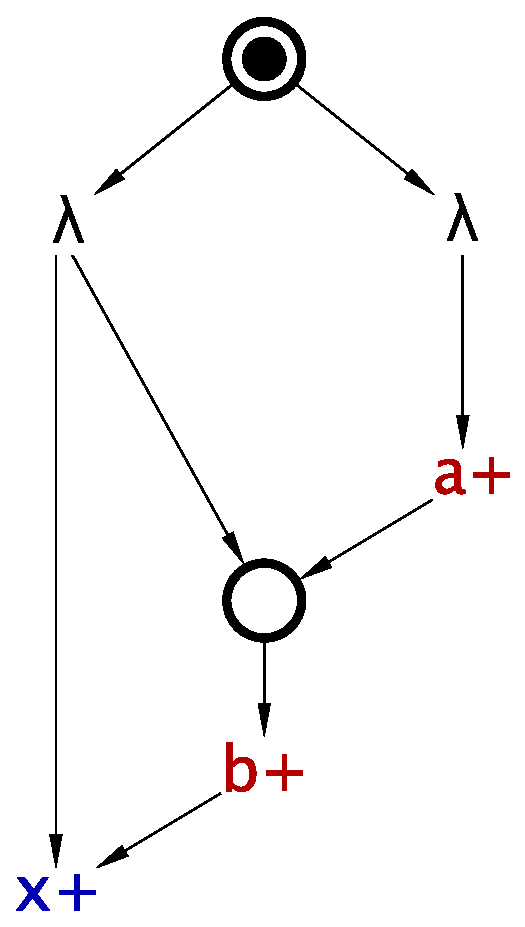
\includegraphics[scale=0.3]{EXPERIMENTS/stg/dummy_counterexample}%
    \hfill%
    \raisebox{5.9em}[5.9em][0em]{\Large$\Rightarrow$}
    \hfill%
    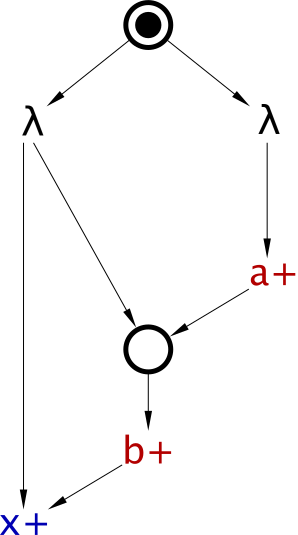
\includegraphics[scale=0.3]{EXPERIMENTS/stg/dummy_counterexample_removed}%
    \hfill%
    {}
    \caption[Example of invalid place removal]{\label{fi-dummy-counterexample}
        Example of an STG where removal of places in the postset of dummy transitions results in a wrong behaviour.
    }
\end{figure}

\section{Proof of Proposition \ref{pr-main}}

We begin with defining the witness $R$ for simulation of $C$ by $C'$.
We say that $(M,M') \in R$ iff $M$ is reachable in $C$ and 
for all places $p \in P'$, $M(p)=M'(p)$.
Note that since $C'$ can be obtained from $C$ by removing places, $P' \subseteq P$ so $M(p)$ is always defined.
Also note that for any given reachable marking $M$ there is exactly one $M'$ such that $(M,M') \in R$, obtained by 
restricting the domain of $M$, so $R$ is a function and we employ the notation $M' = R(M)$ to use it as such.

Now we need to prove that the introduced relation $R$ is indeed bisimulation. 
We'll start by proving that $C'$ simulates $C$ with $R$.
To prove that we first need to show $M'_N = R(M_N)$. That follows from both parallel composition and place removal preserving initial markings of individual places.
Now given a reachable marking $M^1$ with an enabled transition $M^1 \ifrs {l} M^2$ we must show that $R(M^1) \ifrs {l} R(M^2)$. To prove that we note that any transition enabled in $M^1$ must also be enabled in $R(M^1)$ because the enabledness condition gets weakened with removal of places. Using that fact we show that whichever transition $t$ labelled $l$ was enabled to allow $M^1 \tfrs t M^2$ it is also enabled in $R(M^1)$. The marking after firing must coincide with $R(M^2)$ because the arcs to existing places and their weights are preserved by place removal. This shows $R(M^1) \ifrs {l} R(M^2)$ and concludes the proof that $C'$ simulates $C$.

In the second part of the proof we show that $C$ simulates $C'$. Here, given $R(M^1) \ifrs {l} M'^2$ we need to show that there exists a $M^2$ such that $M^1 \ifrs {l} M^2$ and $M'^2 = R(M^2)$. Again, we note that there must be a transition $t'$ labelled $l$ such that $R(M^1) \tfrs t' M'^2$. If the corresponding transition $t$ is enabled $M^1 \tfrs t M^2$ then the proof is complete since we already showed that $M'^2$ must be equal to $R(M^2)$. For the sake of contradiction suppose $t$ is not enabled in marking $M^1$. Then there is necessarily one of the deleted places $p$ in $\pre{t}$ in some of the component STGs $C_i$, and the number of tokens in this place at marking $M^1$ is
smaller than the weight of the arc $(p,t)$ in $C_i$ (*)
Since by condition~\ref{only-inputs-in-postset} $\post{p}$ can
contain only input transitions, $t$ must be labelled by
$s^\pm$, where $s$ is an input signal of $C_i$; \wlogg, we
assume that the label is $s^+$. By
condition~\ref{exists-matching-output} there is also a
component STG $C_j$ where $s$ is an output signal.

Let $\sigma$ be an execution of $C$ terminating at marking $M^1$,
and $\nu$ be the trace corresponding to $\sigma$ (note that
such a $\sigma$ always exists as we restrict $R$ to only include reachable markings).
We proceed by showing that (i)
$\nu|_{C_j}s^+$ is a trace of $C_j$ and (ii) $\nu\, s^+$ is not
a trace of $C$; these would mean that there is a violation of
FCI in the original composition, leading to a contradiction.

(i) Since $s^+$-labelled transition $t'$ is enabled in marking $R(M^1)$ of $C'$, 
its component $t_j$ must be also be enabled in $C_j'$ and labelled by the same signal $s^+$.
Since $s$ is an output in $C_j$, no places were removed from $\pre{t_j}$ when building
$C_j'$ due to condition~\ref{only-inputs-in-postset}, which
means that $t_j$ is also enabled by the marking $M^1_j$, and so $\nu|_{C_j}s^+$
is a trace of $C_j$.

(ii) For the sake of contradiction, suppose $\nu\,s^+$ is a
trace of $C$. Due to the output-determinacy of $C$, the set of
outputs by which $\nu$ can be extended is uniquely determined,
and so $s^+$ must be enabled by $M^1$ (perhaps, after firing
several dummy transitions). By
condition~\ref{injective-labelling} there is only one
$s^+$-labelled transition in $C_i$ (\viz $t$), and so each
$s^+$-labelled transition in $C$ has $p$ in its preset with the
arc from $p$ to this transition having the same weight as the
arc $(p,t)$ in $C_i$. Consequently, each $s^+$-transition in
$C$ is blocked at marking $M^1$ because by (*) the number of tokens
in $p$ is smaller than the weight of the corresponding arc.
Moreover, firing only dummy transitions cannot increase the
number of tokens in $p$ and thus enable an $s^+$-labelled
transition, as by condition~\ref{no-dummies-in-preset}
$\pre{p}$ contains no dummy transitions, a contradiction. Hence
$\nu\,s^+$ is not a trace of $C$.

As explained above, (i) and (ii) imply a violation of FCI and
so lead to a contradiction, which means that $C$ and
$C'$ must be bisimilar.

\section{Discussion}

In practice, when performing the parallel composition, one
would like as few implicit places as possible in the result,
and so it would be desirable to weaken the conditions in
Prop.~\ref{pr-main}, so that as many places as possible are
removed. As the conditions~\ref{only-inputs-in-postset}
and~\ref{exists-matching-output} are intrinsic, it is unlikely
that they can be relaxed. However, the technical
conditions~\ref{injective-labelling}
and~\ref{no-dummies-in-preset} can be dealt with --- by
ensuring that the components always satisfy them. Indeed, as
mentioned in Sect.~\ref{sec_pn_basic}, for output-determinate
STGs the language is the semantics, and so one often can remove
dummy transitions and enforce injective labelling without
changing the language, \eg using the \petrify
tool~\cite{ckkly97}; this will ensure that
conditions~\ref{injective-labelling}
and~\ref{no-dummies-in-preset} hold. An example of such a
transformation for the \balsa standard component Call is shown
in Fig.~\ref{fi-enforce-inj}. This operation is performed on
(small) components rather than the (large) composition, and so
is usually cheap. Moreover, in some applications, in particular
circuit re-synthesis, the components are taken from a fixed
library of component types, and so the transformation can be
performed only once for each component type, and subsequently
incur no runtime penalty at all.

\begin{figure}[!tb]
    \centering
    {}%
    \hfill%
    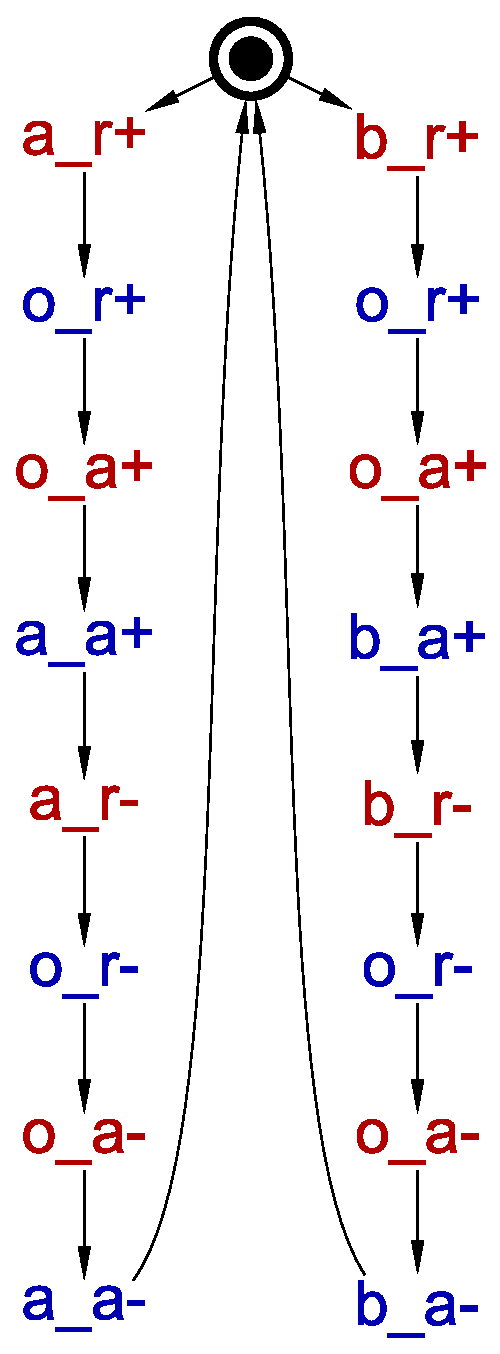
\includegraphics[scale=0.3]{EXPERIMENTS/stg/mix_full}%
    \hfill%
    \raisebox{8.9em}[8.9em][0em]{\Large$\Rightarrow$}
    \hfill%
    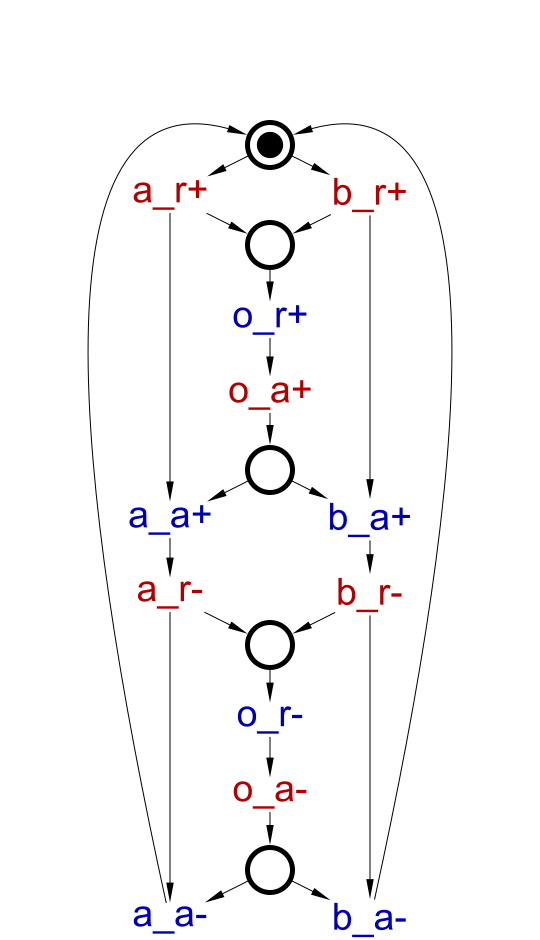
\includegraphics[scale=0.3]{EXPERIMENTS/stg/mix_full_inj}%
    \hfill%
    {}
    \caption{\label{fi-enforce-inj}
        Example of enforcing injective labelling in an STG.
    }
\end{figure}

\section{Experiments}\label{se-exp}

\begin{figure*}[!tb]
\centering
    \phantom{\,}%
    \hfill%
    $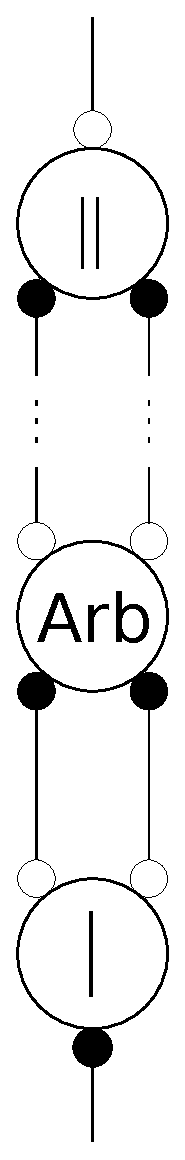
\includegraphics[scale=0.3]{fig/par_arb_mix}
    \atop
    \mbox{\rule[1.3em]{0em}{0em}\ParArbCall}$%
    \hfill%
    $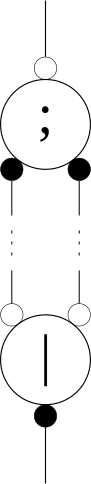
\includegraphics[scale=0.3]{fig/seq_mix}
    \atop
    \mbox{\rule[1.3em]{0em}{0em}\SeqCall}$%
    \hfill%
    $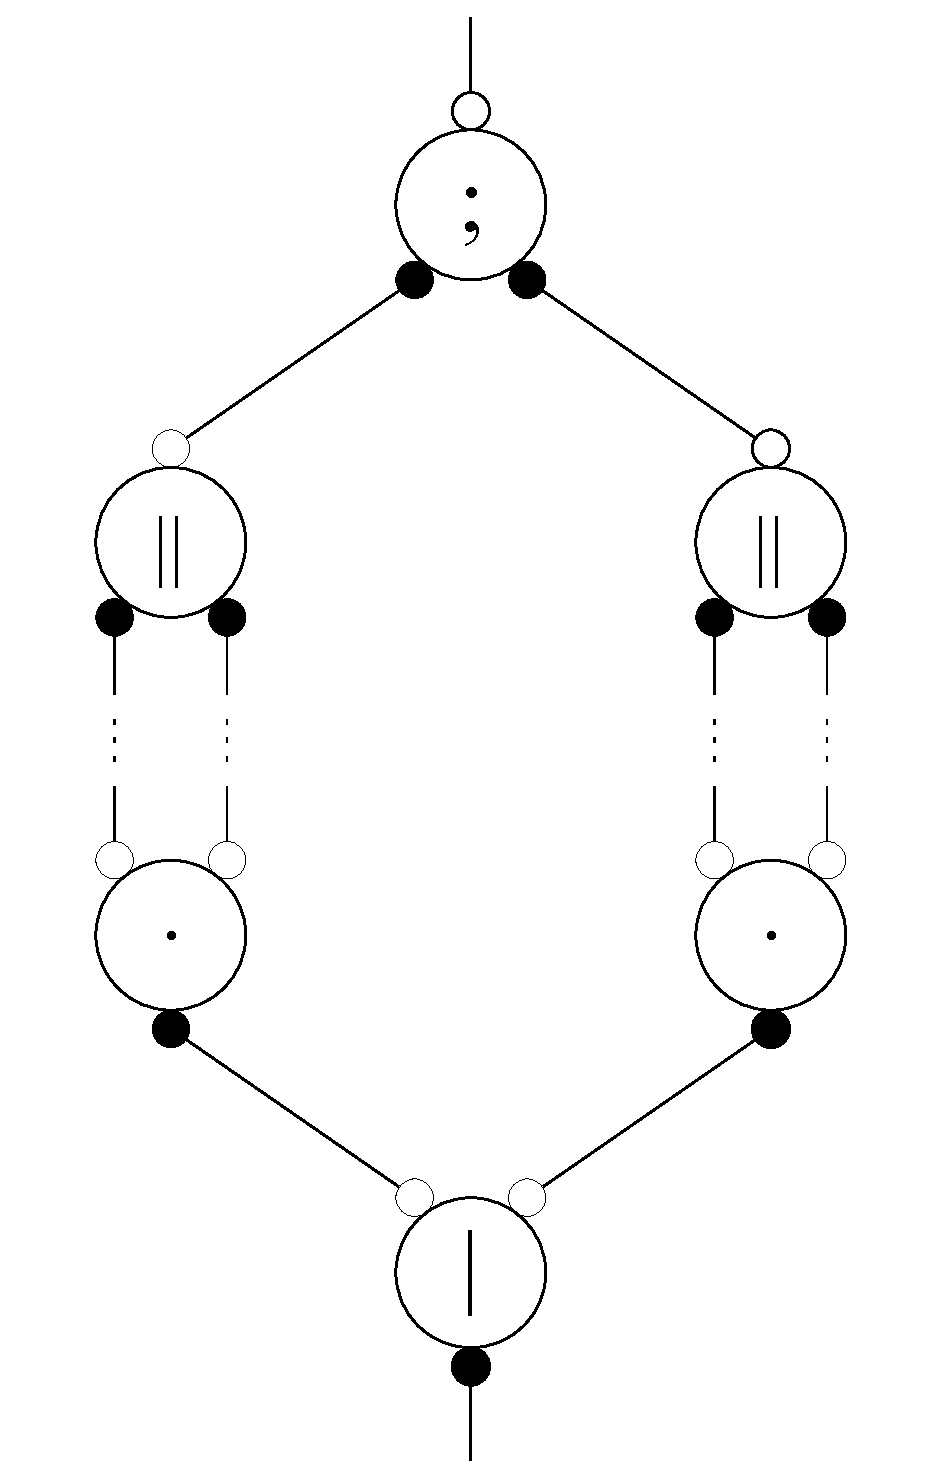
\includegraphics[scale=0.3]{fig/seq_par_sync_mix}
    \atop
    \mbox{\rule[1.3em]{0em}{0em}\SeqCallParSync}$%
    \hfill%
    \phantom{\,}%
    \\
    \caption{\label{fig:Scalable-Balsa-controllers}
        Scalable Balsa controllers used in experiments.
    }
\end{figure*}

\begin{figure*}[p]
\centering

  \subfloat[All contractions]{
    \shortstack[l]{
    $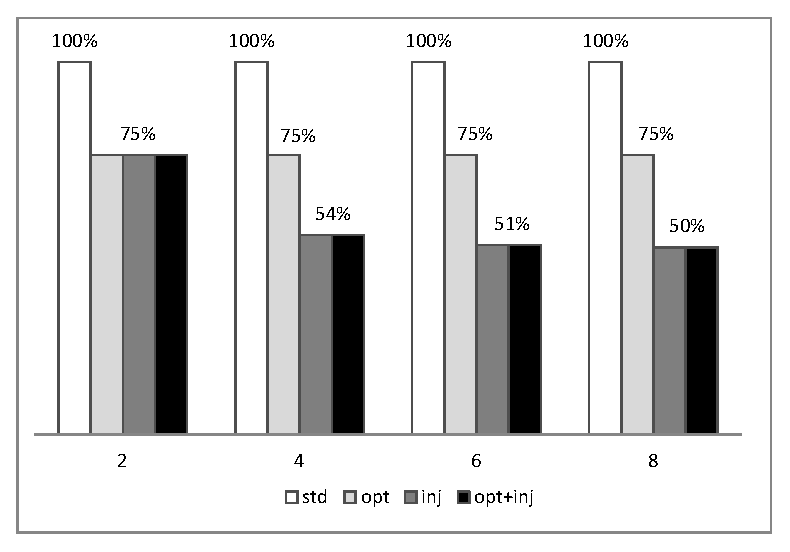
\includegraphics[width=0.48\textwidth]{fig/ParArbMix_all}
    \atop
    \mbox{\rule[1.3em]{0em}{0em}\ParArbCall}$%
    \\[1em]
    $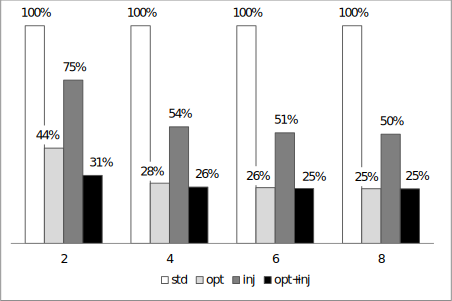
\includegraphics[width=0.48\textwidth]{fig/SeqMix_all}
    \atop
    \mbox{\rule[1.3em]{0em}{0em}\SeqCall}$%
    \\[1em]
    $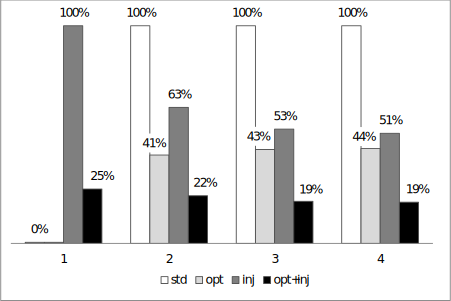
\includegraphics[width=0.48\textwidth]{fig/SeqMixParSync_all}
    \atop
    \mbox{\rule[1.3em]{0em}{0em}\SeqCallParSync}$%
    }
    }
    \hfill%
  \subfloat[Safeness-preserving contractions]{
    \shortstack[l]{
    $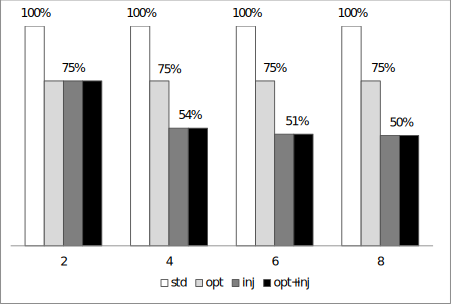
\includegraphics[width=0.48\textwidth]{fig/ParArbMix_safe}
    \atop
    \mbox{\rule[1.3em]{0em}{0em}\ParArbCall}$%
    \\[1em]
    $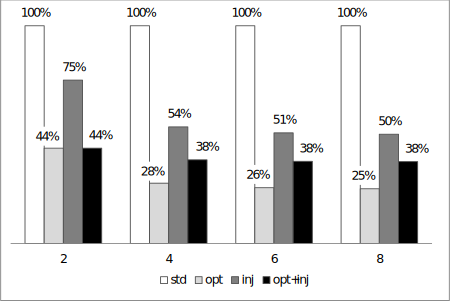
\includegraphics[width=0.48\textwidth]{fig/SeqMix_safe}
    \atop
    \mbox{\rule[1.3em]{0em}{0em}\SeqCall}$%
    \\[1em]
    $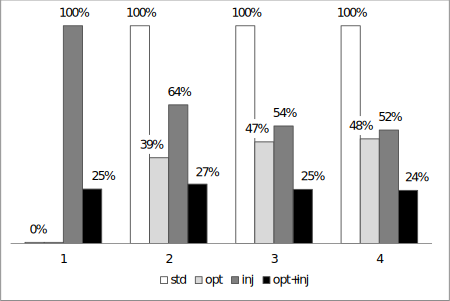
\includegraphics[width=0.48\textwidth]{fig/SeqMixParSync_safe}
    \atop
    \mbox{\rule[1.3em]{0em}{0em}\SeqCallParSync}$%
    }}
    \caption{\label{fi-exp}
        Experimental results.
    }
\end{figure*}

The proposed parallel composition algorithm has been evaluated
on three series of scalable benchmarks (available
from~\cite{pcomp}), see
Fig.~\ref{fig:Scalable-Balsa-controllers}. They are built of a
subset of standard \balsa components~\cite{EB-02}:
Paralleliser~$(\parallel)$, Sequencer~$(;)$, Call~$(|)$,
Synchroniser~$(\cdot)$ and Arbiter~(Arb). These controllers are
considered to be of size~1; a controller of size~$k>1$ is
constructed by replacing the dotted lines with the controllers
of size~$k-1$. Each basic component is described by an
individual STG; then these STGs are composed using four
different techniques:
\begin{description}
  \item[std] the standard parallel composition;
  \item[opt] the optimised parallel composition presented
      here;
  \item[inj] the standard parallel composition of the
      components with enforced injective labelling;
  \item[opt+inj] the optimised parallel composition of the
      components with enforced injective labelling.
\end{description}
Note that all the used \balsa components except Call initially
had injective labelling, so only the STG for Call was changed
in the inj and opt+inj series. Both the standard and optimised
parallel composition algorithms have been implemented in \pcomp
tool~\cite{pcomp}. The tool automatically deletes duplicate
places in all compositions, so all the experimental results are
subject to this simplification. The runtimes of \pcomp were
negligible and so not reported.

For each composed STG, the internal signals of the composition
were hidden (\ie turned into dummies), and the \desij
tool~\cite{DesiJ} was used to structurally eliminate as many
dummies as possible, using either secure or safeness-preserving
secure contractions.

The results of our experiments are summarised by the charts in
Fig.~\ref{fi-exp}. There are six charts altogether, for each of
the three benchmark series and each of the contraction modes
(secure or safeness-preserving secure). Each chart reports, for
each benchmark size within the corresponding series, the
numbers of non-con\-trac\-tible dummy transitions (normalised
\wrt the worst result) remaining in the STG for each of the
four composition methods described above.

The experiments demonstrate that the optimised parallel
composition is never worse than the standard one in terms of
the STG structure that is used for removing dummies (the opt
bars are never longer than the std bars, and the opt+inj bars
are never longer than the inj bars), and is significantly
better in some cases (\eg for the \SeqCallParSync(4) benchmark
there is a factor of five improvement). Moreover, using the
optimised technique in conjunction with injective labelling is
usually advantageous (the fourth bar is the shortest in almost
all cases).

\section{Balsa workflow optimisation through STG resynthesis}

\label{sec:balsa-workflow}

\begin{figure}
\begin{centering}
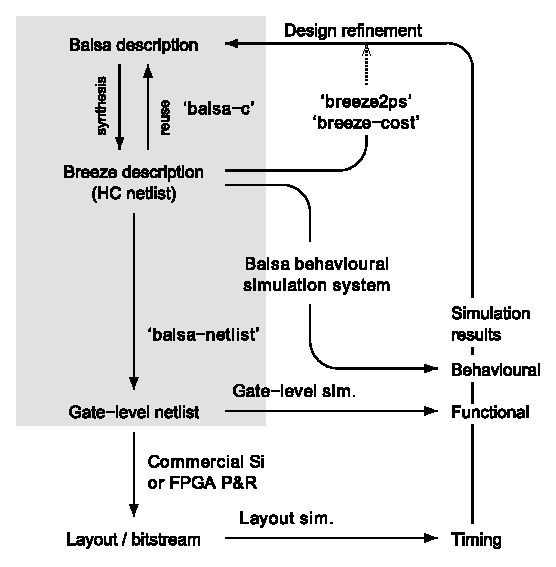
\includegraphics[width=0.40\paperwidth]{figures/balsa-design-workflow}
\par\end{centering}

\centering{}\caption{Balsa design workflow\label{fig:Balsa-design-workflow}}
\end{figure}


\begin{figure}
\begin{centering}
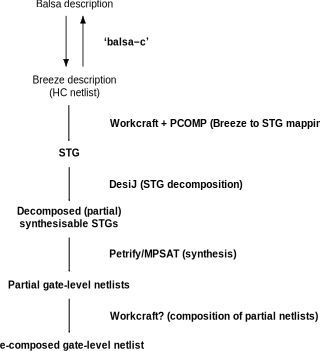
\includegraphics[width=0.40\paperwidth]{figures/balsa-workflow-modification}
\par\end{centering}

\caption{Modified Balsa workflow\label{fig:Modified-Balsa-workflow}}
\end{figure}


The standard Balsa design workflow is comprised of several stages~(Figure~\ref{fig:Balsa-design-workflow}).
The designer writes the system specification in Balsa language. It
is passed to the Balsa compiler, which generates a handshake component
netlist (produced in a language called Breeze) using syntax-directed
mapping on the source code. Syntax-directed mapping in this context
means that there is a predefined handshake component construct for
every syntactic structure. The Breeze netlist is then translated into
a gate-level netlist using direct mapping, this time from individual
handshake components to their gate-level implementation, which is
defined beforehand.

The proposed modification of this workflow is shown in~Figure~\ref{fig:Modified-Balsa-workflow}.
The translation from Balsa language into Breeze netlist is retained
(and is still done by the Balsa compiler), but the Breeze-netlist
to gate-level-netlist mapping is replaced with the STG resynthesis
flow as introduced in section~\ref{sec:Balsa-Introduction}. Instead of
using Balsa tools to produce a gate-level netlist, the Breeze netlist
is read by a special interpreted graph model plug-in to \noun{Workcraft
}tool~\cite{DBLP:conf/apn/PoliakovKY09}, which replaces the handshake
components with their STG specifications and produces a composition
of those STGs using \noun{PComp} tool. If the resulting STG is small
enough, the gate-level implementation may immediately be synthesised
using any of the available synthesis tools.

However, for many practical cases the composed STG will become quite
large. In this case, to synthesise the implementation it is necessary
to insert an additional decomposition step, which may be either STG
decomposition~(implemented using a tool called \noun{DesiJ~}\cite{DesiJ}
that is automatically called from the plug-in), or\noun{ }handshake
circuit~(HC) decomposition which is supported by the plug-in directly.
Therefore, the whole process is automated in the \noun{Workcraft }framework.

The technique allows to synthesise more efficient control circuits
while at the same time preserving the benefit of rapid design methodology
fundamental to Balsa. It should be noted, however, that full modelling
of all Breeze components with STGs is not practical. The behaviour
of most data components would be too complex to synthesise from an
STG. Circuit resynthesis for such components would take too much time
and would often be less effective than an already existing gate-level
implementation done by an experienced designer. Subsequently, all
data-related functionality in HCs is modelled outside of STG composition
framework: the STG models include only control signals for the data
path elements. These control signals are to be connected after the
gate-level generation step to the data-path circuit that is assembled
separately (its components are specified by a structural Verilog netlist).
The data path is generated automatically side-by-side with the STG
behaviour model.


\section{Support of Breeze Handshake Circuits as Interpreted Graph Model in
\noun{Workcraft}}

For the purpose of implementation of the design flow discussed in
this section the \noun{Workcraft} framework was extended with a plug-in
that introduces support for Breeze HCs. The new HC model allows \noun{Workcraft}'s
convenient visual editing tools to be applied for creation and editing
of Breeze netlists. The same plug-in also performs generation of the
STG behaviour model for the specified HC. The STG generation algorithm
is designed to be highly customisable, with support of multiple handshake
protocols and various STG implementations for each type of component.
At the moment of writing, STG generation was implemented for a limited
set of components using early 4-phase handshake protocol. The library
of components is being expanded and will include all Breeze components
with support for different handshake protocols.


\section{STG specifications of individual handshake components\label{sec:Individual-component-examples}}

Balsa components can be roughly divided in three groups: pure control
components, data path control components and data-control interface
components. We will review each group separately.


\subsection{Pure control path components}

\newcommand{\vcent}[1]{
  $\vcenter{\hbox{#1}}$
}
\newcommand{\balsafigSZ}[1]{
\vcent{\includegraphics[scale=0.6]{#1}}
}

\begin{figure}

\subfloat[Sequence\label{fig:SequenceOptimised}]{
\centering
\balsafigSZ{figures/Control/sequence-HC}
~~
\vcent{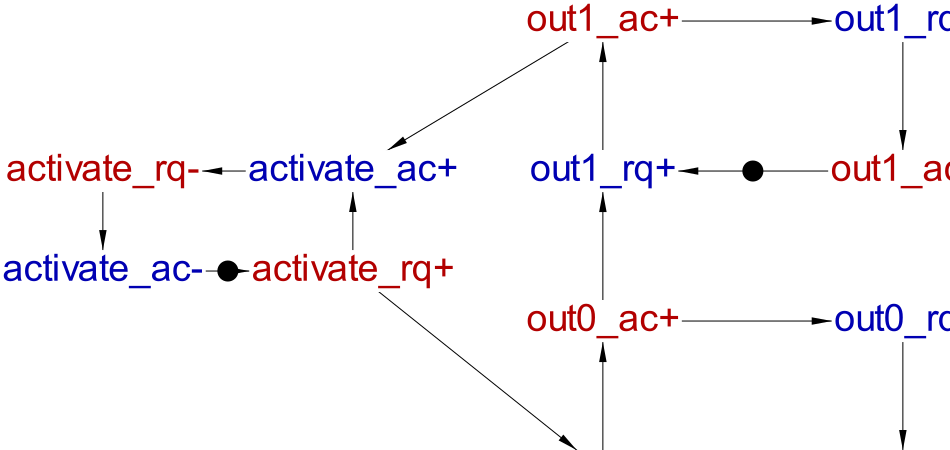
\includegraphics[scale=0.25]{figures/Control/sequenceoptimised}}
}

\subfloat[Concur\label{fig:Concur}]{
\centering
\balsafigSZ{figures/Control/concur-HC}~~\vcent{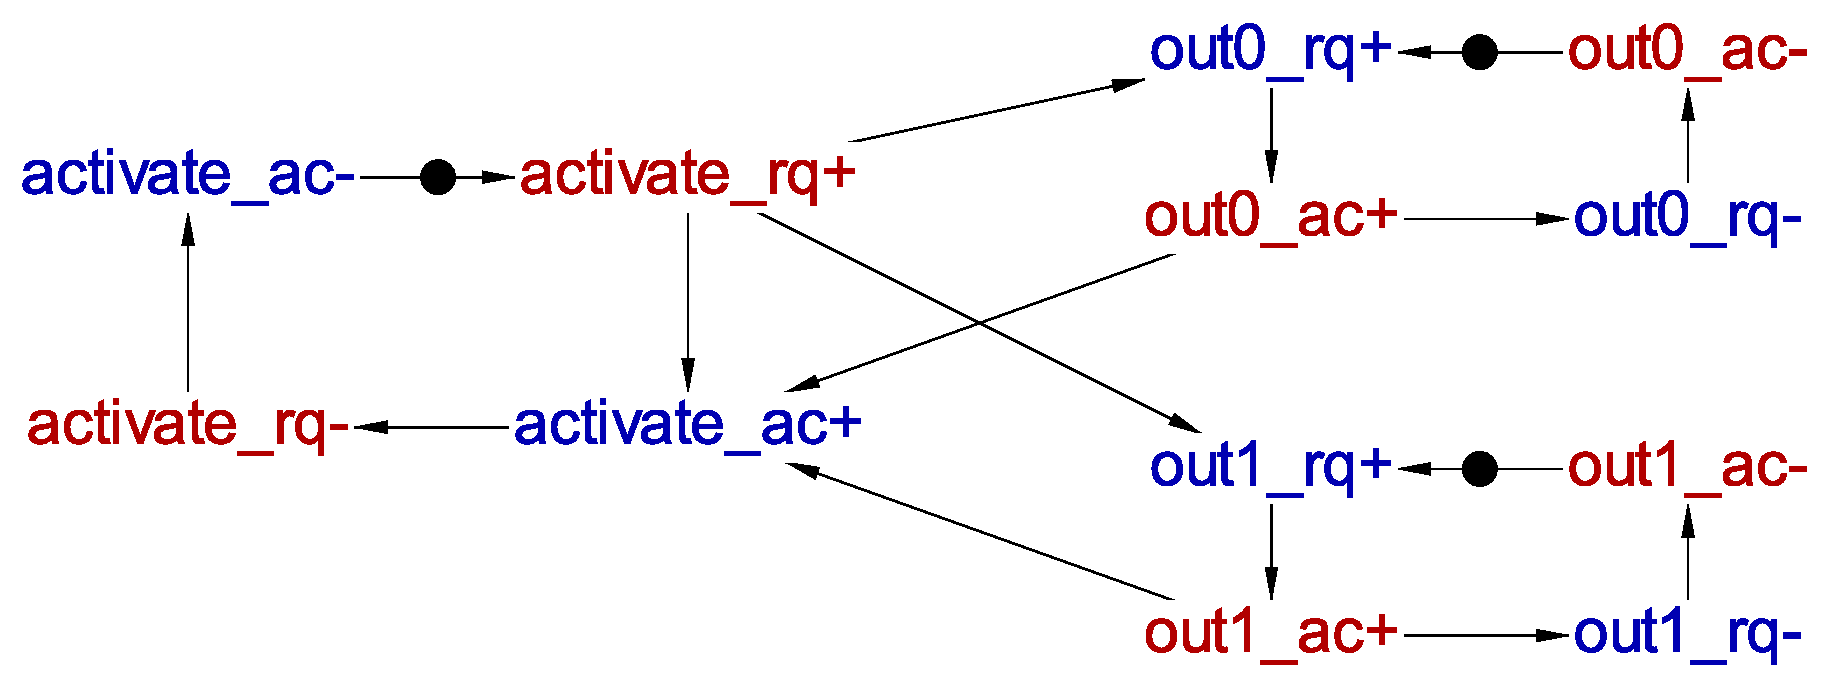
\includegraphics[scale=0.25]{figures/Control/concur}}
}

\caption{Pure control path handshake components and their respective STGs}
\end{figure}


Pure control components only control the behaviour of other components
and do not carry out any data operations. These components are expected
to gain the most from the new design workflow because all of their
handshakes are inside the control path and such handshaking does not
have to always strictly correspond to the general protocol.

The examples are Concur~(Figure~\ref{fig:Concur}) and SequenceOptimised~(Figure~\ref{fig:SequenceOptimised})
components. The STGs in those figures are highly parallel specifications
of these components. However, experimental results show that although
such implementation might look better on paper, in practise it is
sometimes better to specify traditional, more sequential behaviour.
This significantly simplifies the task for synthesis tools, particularly
those based on state space exploration techniques, because high parallelism
often leads to early state space explosion problem. Besides that,
a parallel specification suffers more from CSC~(complete state coding)
problems: a significant number of auxiliary signals have to be introduced
to achieve CSC.


\subsection{Data path control components}

\begin{figure}
\subfloat[BinaryFunc\label{fig:BinaryFunc}]{\begin{centering}
\balsafigSZ{figures/Data/binaryfunc-HC}~~\vcent{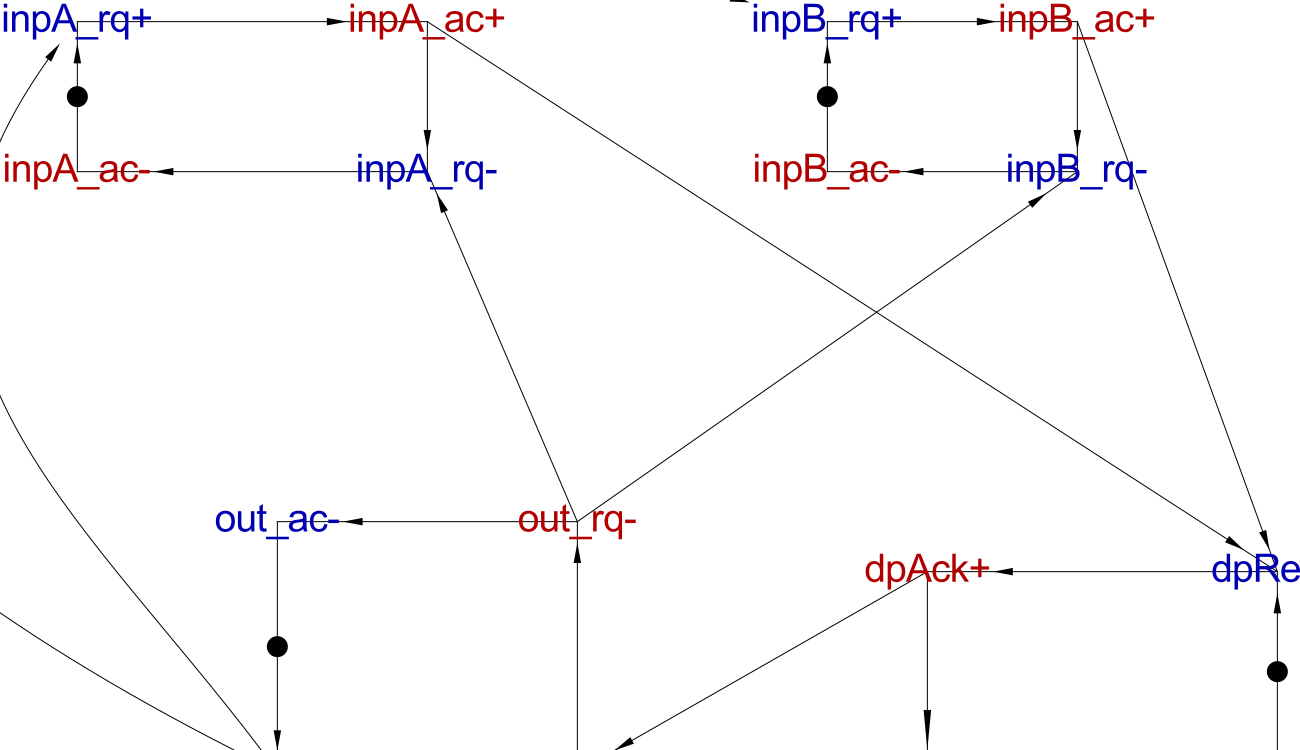
\includegraphics[scale=0.25]{figures/Data/binaryfunc}}
\par\end{centering}

}

\subfloat[CallMux\label{fig:CallMux}]{\begin{centering}
\balsafigSZ{figures/Data/callmux-HC}~~\vcent{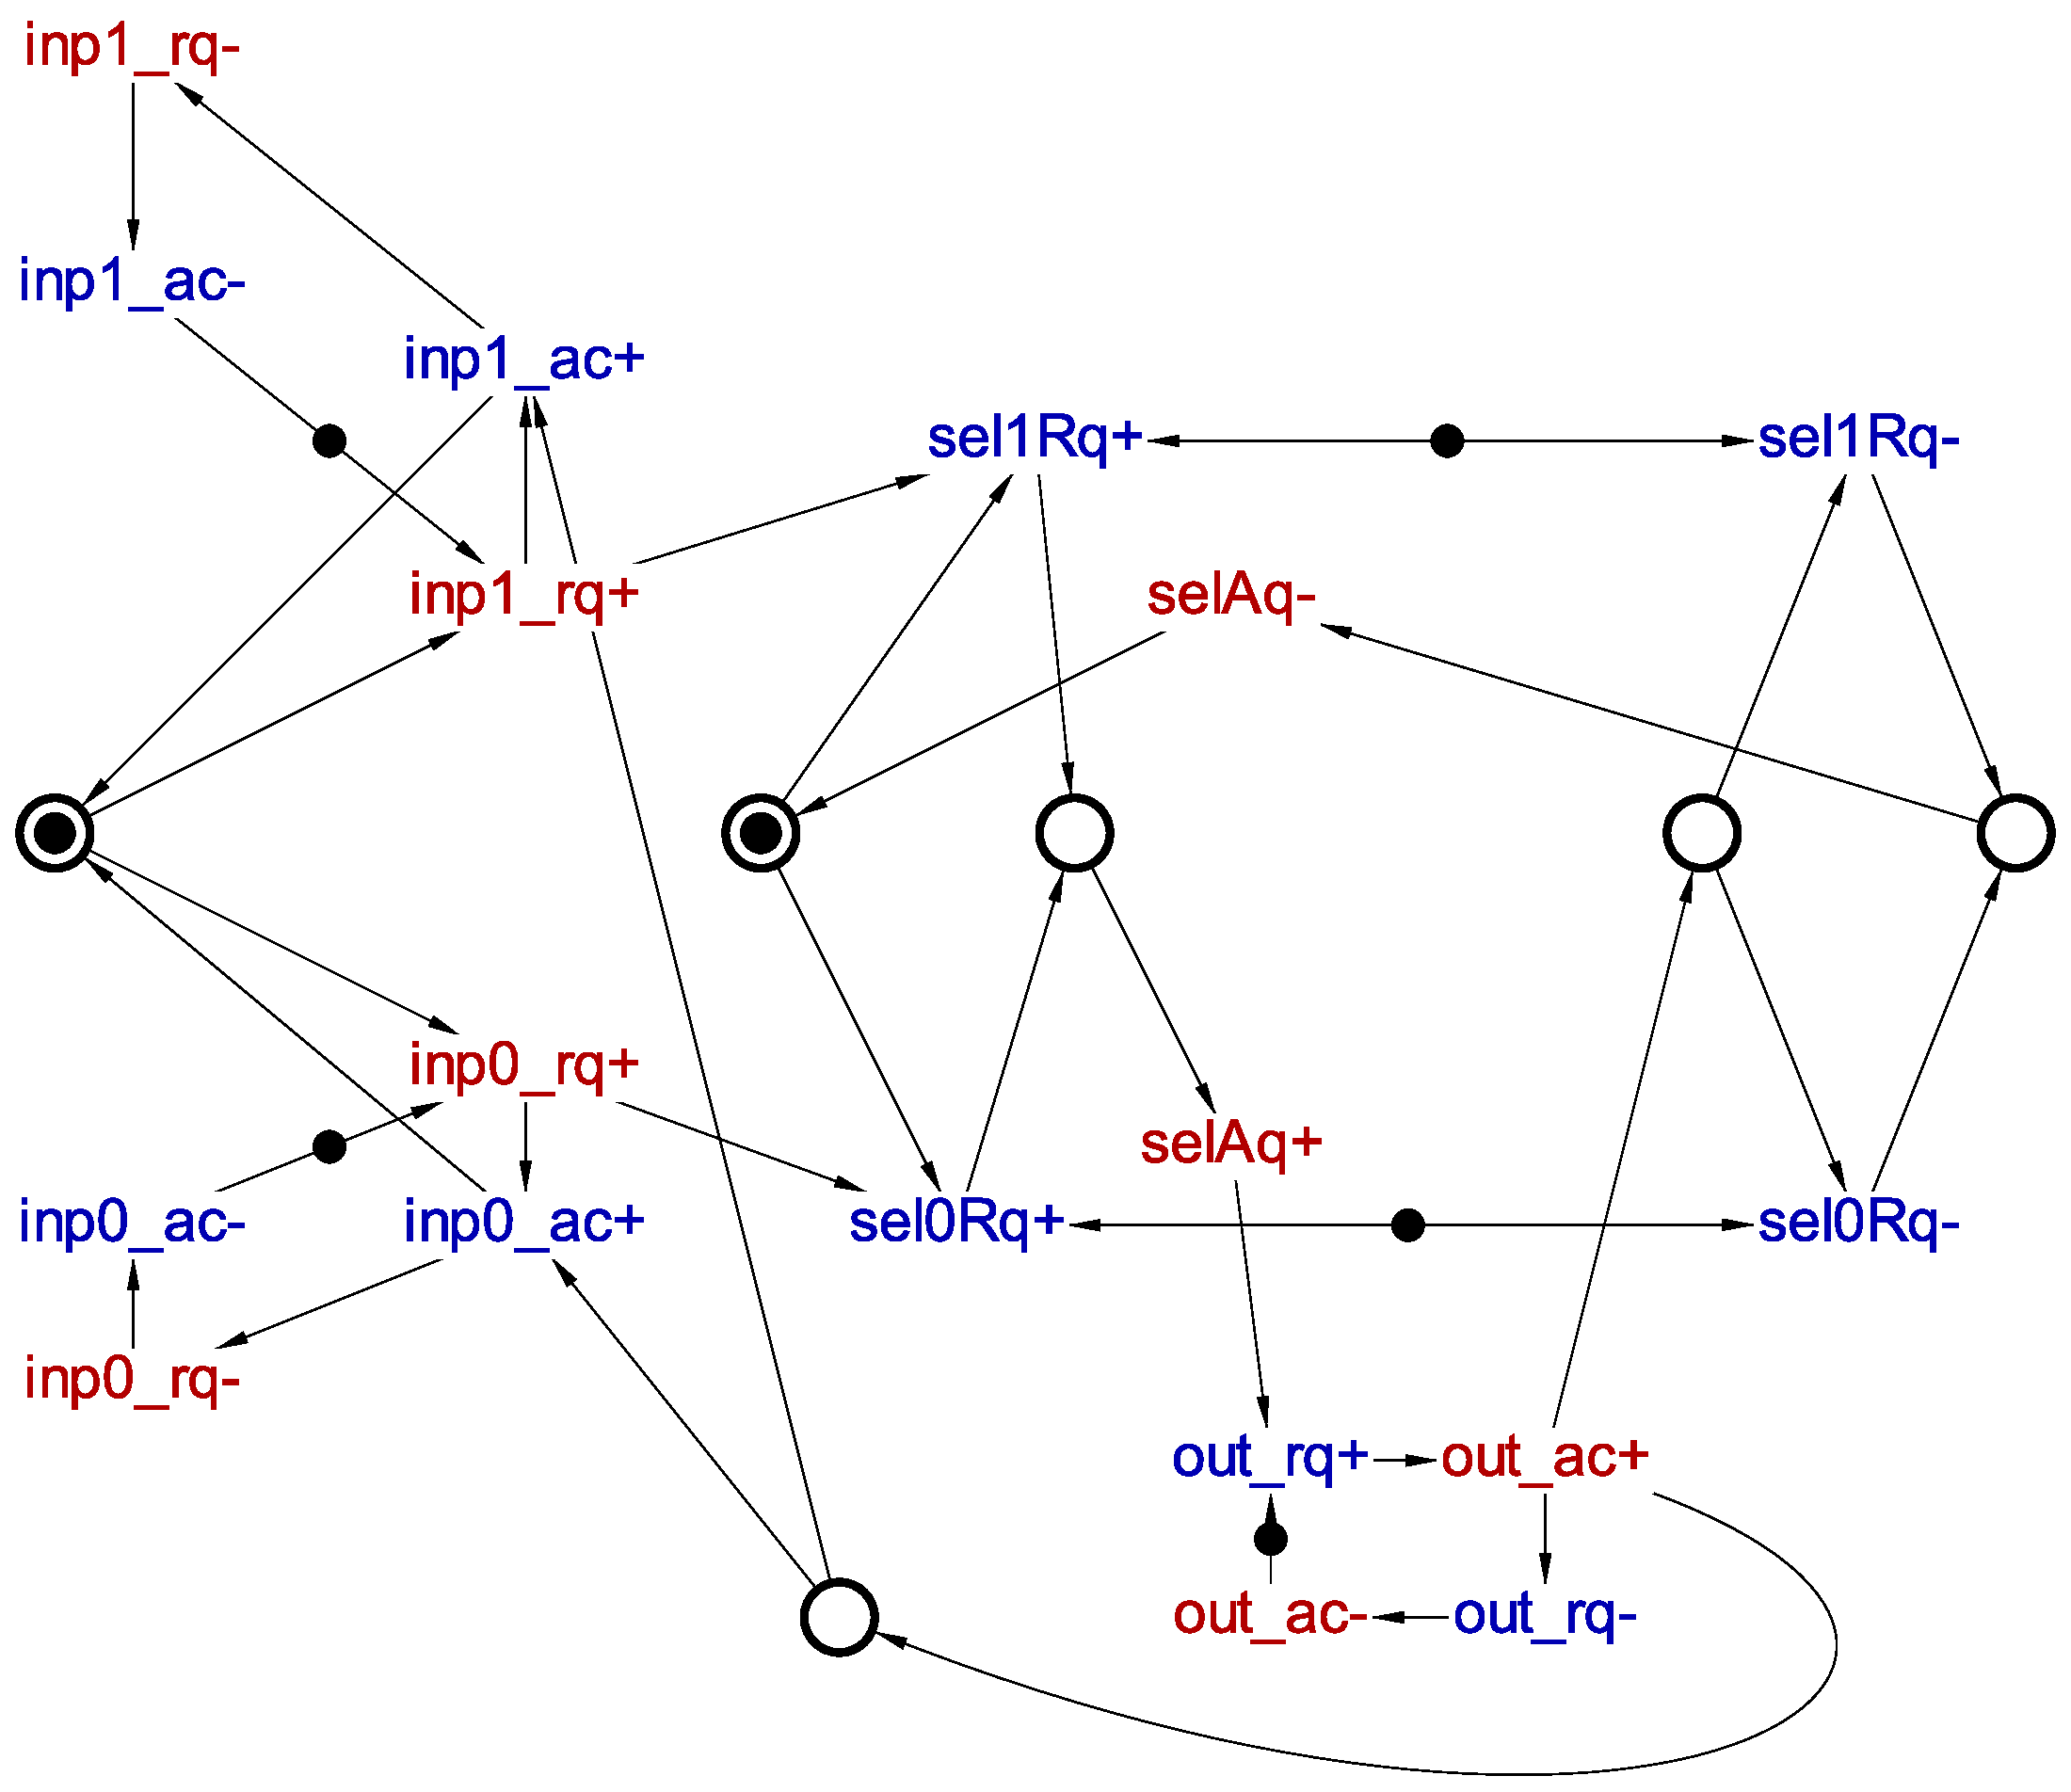
\includegraphics[scale=0.25]{figures/Data/callmux}}
\par\end{centering}

}

\subfloat[Variable\label{fig:Variable}]{\begin{centering}
\balsafigSZ{figures/Data/variable-HC}~~\vcent{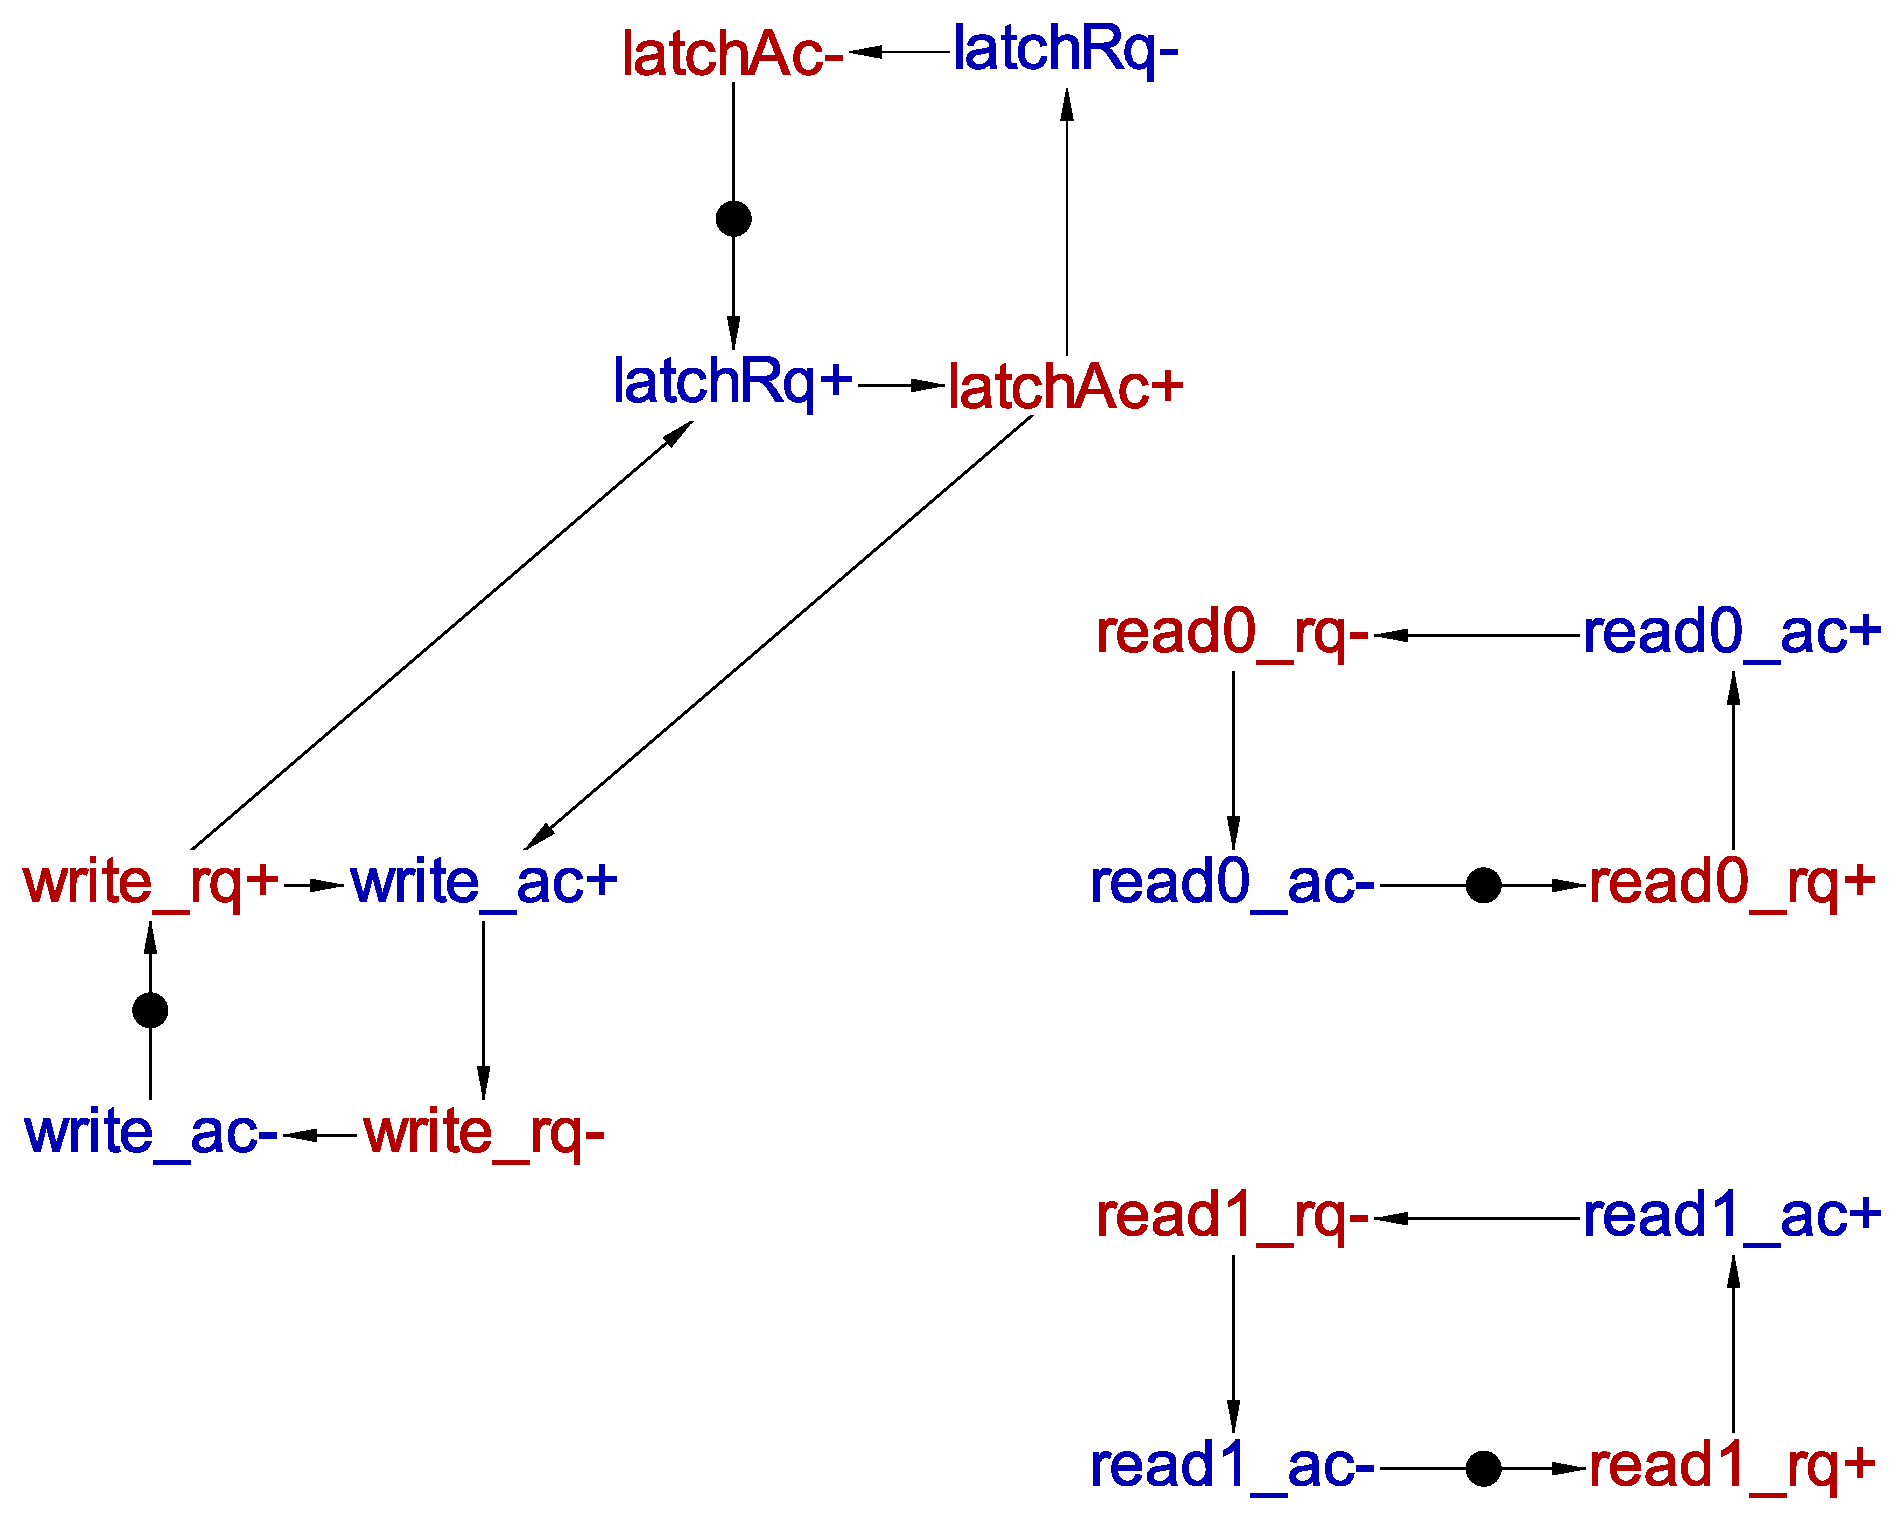
\includegraphics[scale=0.25]{figures/Data/variable}}
\par\end{centering}

}

\caption{Pure control path handshake components and their respective STGs}
\end{figure}


This group of components is used to control the the corresponding
data path components that execute predefined operations on data. These
operations are far too complex for automated synthesis, but the control
path part can still be optimised using STG resynthesis, which makes
it reasonable to separate data and control signals. The signals that
control the data path are in this case specified as the input and
output signals of the component's STG. Because the data path blocks
are outside this specification, their handshake protocols must be
implemented strictly and thus cannot be optimised. This, however,
does not prevent the optimisation of handshakes that belong to the
same component but interface with other control path components.

BinaryFunc~(Figure~\ref{fig:BinaryFunc}), CallMux~(Figure~\ref{fig:CallMux}),
Variable~(Figure~\ref{fig:Variable}) are good examples of the data
path control components.


\subsection{Data-control interface components}

\begin{figure}
\begin{raggedright}
\subfloat[While\label{fig:While}]{\begin{centering}
\vcent{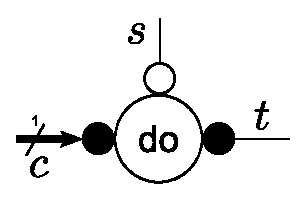
\includegraphics[bb=0bp 0bp 134bp 80bp,scale=0.6]{figures/while-HC}}~~\vcent{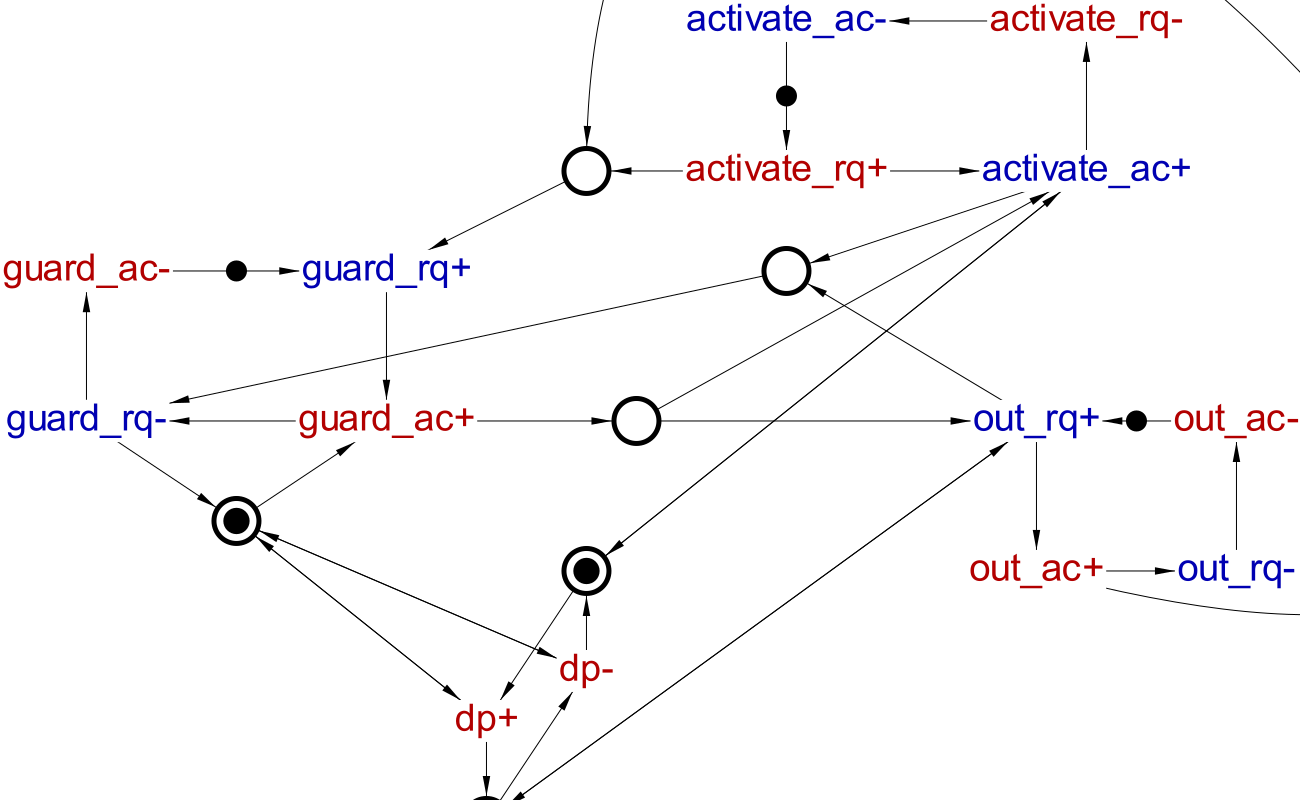
\includegraphics[scale=0.25]{figures/while}}
\par\end{centering}

}
\par\end{raggedright}

\begin{raggedright}
\subfloat[Case\label{fig:Case}]{\begin{centering}
\balsafigSZ{figures/case-HC}~~\vcent{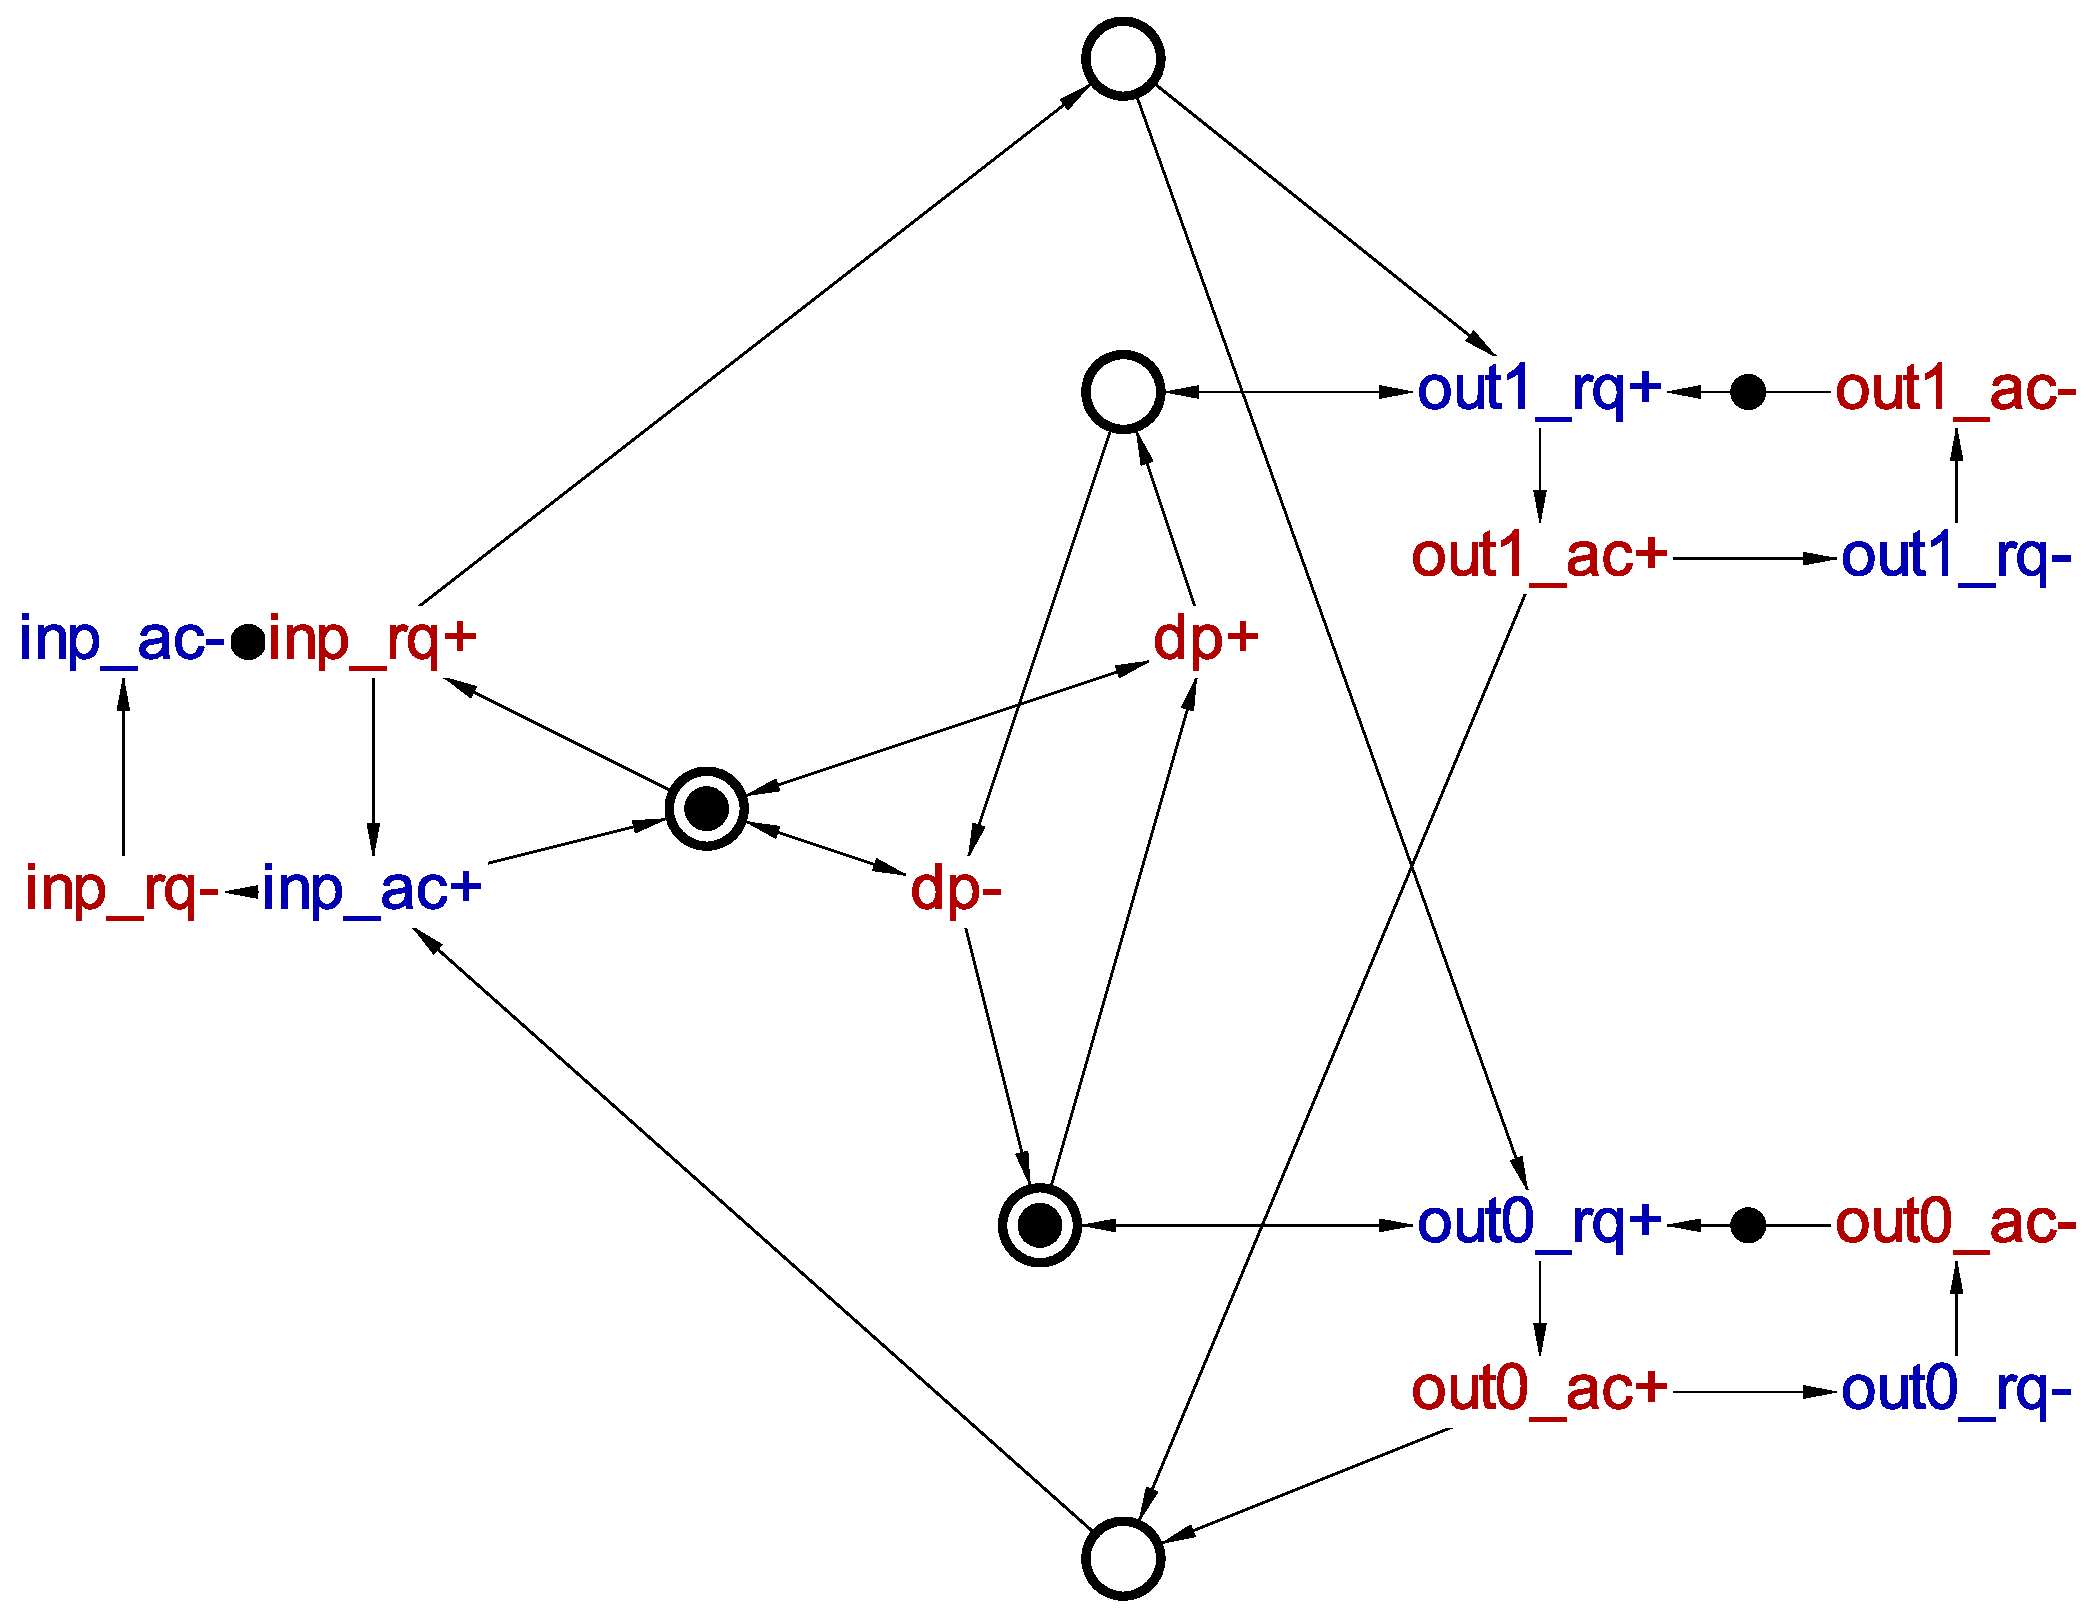
\includegraphics[scale=0.25]{figures/case}}
\par\end{centering}

}
\par\end{raggedright}

\caption{Data-control interface components and their respective STGs\label{fig:Data-control-interface-components}}
\end{figure}


Data-control interface components provide conversion of data to control
signals or vice versa. For example, the While component~(Figure~\ref{fig:While})
analyses the input data to decide whether it should end its operation
and conclude the activation handshake, or to continue activating the
output handshake. Case component~(Figure~\ref{fig:Case}) handles
the data in a very similar way, however it has an arbitrary bus width,
so for bus widths of more than one bit a decoder that resides in the
data path could be used to reduce the STG complexity. These components
STGs can become quite complex and the strict behaviour of their data-path
handshakes must be preserved.


\section{An example: GCD controller}

\begin{figure}[!t]
\begin{centering}
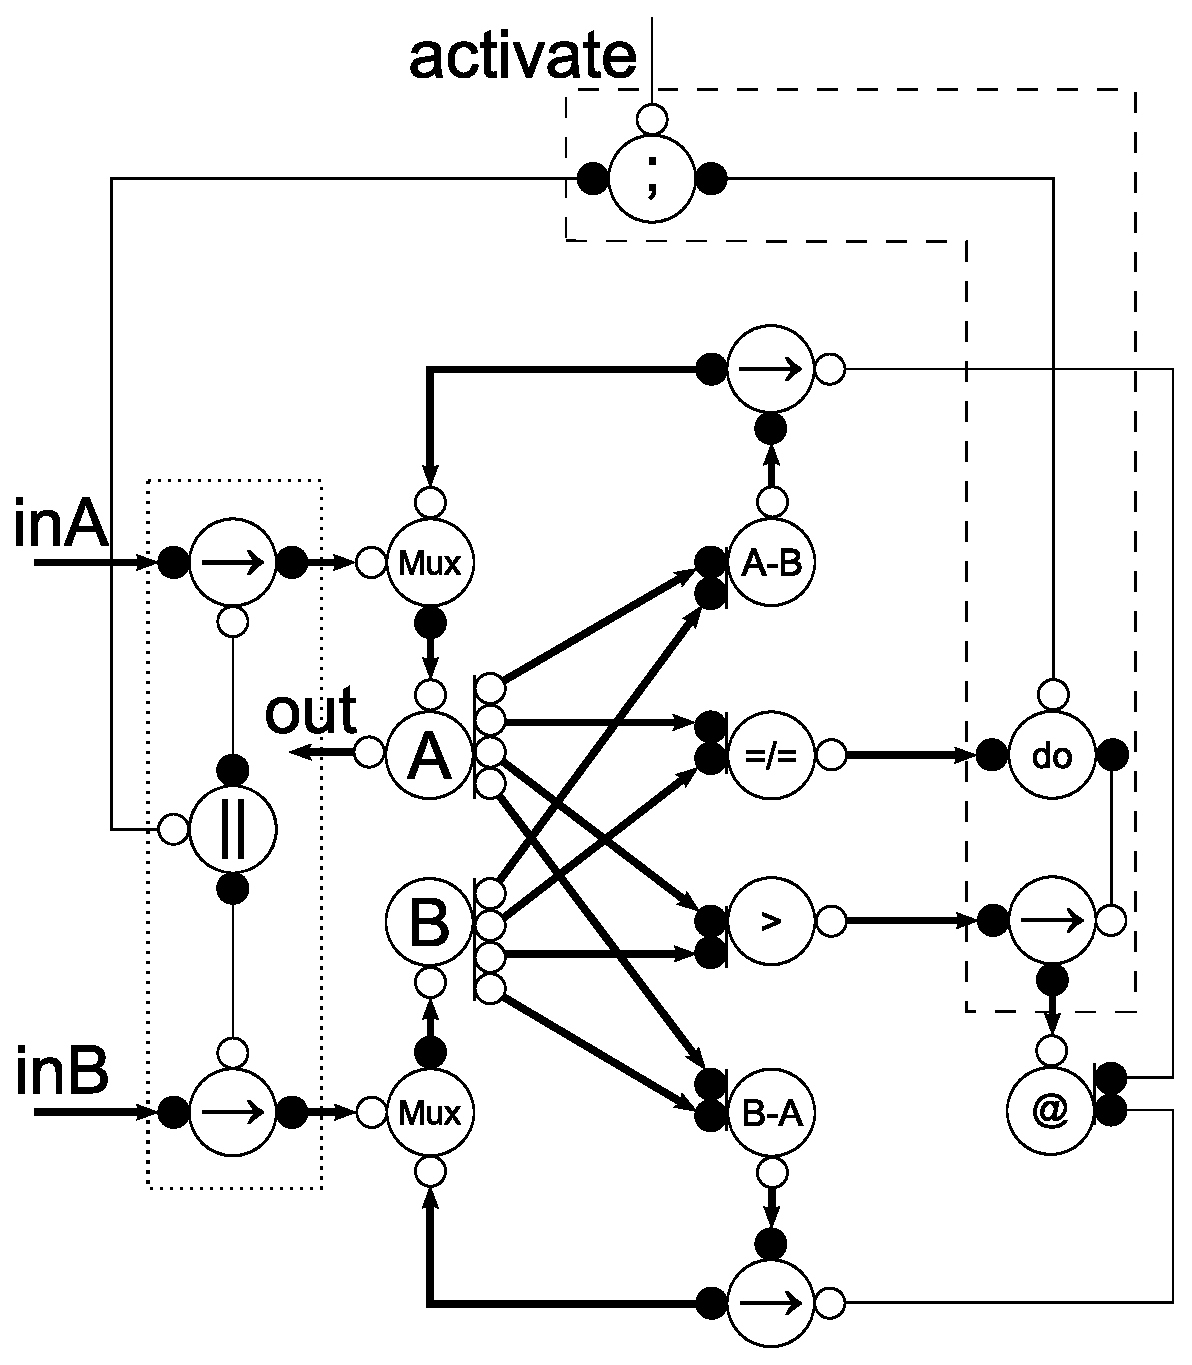
\includegraphics[width=0.3\paperwidth]{figures/breeze-gcd-partition}
\par\end{centering}

\caption{Breeze Handshake Circuit model of a GCD block\label{fig:GCD}}
\end{figure}


We have chosen the GCD controller~(Figure~\ref{fig:GCD}) to demonstrate
how the proposed technique applies to real-life circuits. The GCD
controller is a good research example because it has components from
every group described in section \ref{sec:Individual-component-examples}
and its complexity does not allow omitting of the STG decomposition
step, which is an important part of the proposed workflow. All available
synthesis tools failed to synthesise a circuit from the fully composed
STG model of GCD controller. This proves that the decomposition is
a necessary step lacking which the synthesis of a practical circuit
is not likely to succeed.

Decomposition on the level of STG can be replaced with decomposition
on the level of handshake components. Such decomposition can be done
simply by partitioning the input handshake circuit into blocks, trying
to minimise the number of handshakes between blocks, and applying
the synthesis process to each block separately. While working with
the GCD example it was found that decomposition on the level of handshake
components can be done easier and is guaranteed to be successful,
whereas decomposition on the STG level is a complex task, which requires
additional third-party tools.


\section{Experimental results}

\begin{table}[!t]
\begin{centering}
\begin{tabular}{|c|c|c|c|}
\hline 
Component type & \noun{MPSat} cost & \noun{Petrify} cost & Best\tabularnewline
\hline 
\hline 
BinaryFunc & 21 & 27 & 21\tabularnewline
\hline 
Case & 13 & 13 & 13\tabularnewline
\hline 
Fetch & 17 & 13 & 13\tabularnewline
\hline 
Concur & 16 & 16 & 16\tabularnewline
\hline 
Variable & 13 & 18 & 13\tabularnewline
\hline 
Sequence & 13 & 13 & 13\tabularnewline
\hline 
CallMux & 25 & 33 & 25\tabularnewline
\hline 
While & 17 & 17 & 17\tabularnewline
\hline 
\hline 
\noun{Total} & 305 & 333 & 285\tabularnewline
\hline 
\end{tabular}
\par\end{centering}

\caption{Costs of individual components\label{tab:Costs-of-individual}}


\end{table}


\begin{table}[t]
\begin{centering}
\begin{tabular}{|c|c|}
\hline 
\multicolumn{2}{|c|}{\noun{MPSat}}\tabularnewline
\hline 
Synthesised block & Cost\tabularnewline
\hline 
\hline 
seq+concur+2xfetch & 35\tabularnewline
\hline 
fetch+var+2xBF & 49 \tabularnewline
\hline 
fetch+var+2xBF & 49 \tabularnewline
\hline 
fetch+case & 23 \tabularnewline
\hline 
while & 17 \tabularnewline
\hline 
callmux & 25\tabularnewline
\hline 
callmux & 25\tabularnewline
\hline 
\hline 
\noun{Total}  & 223\tabularnewline
\hline 
\end{tabular}\noun{~~~~}%
\begin{tabular}{|c|c|}
\hline 
\multicolumn{2}{|c|}{\noun{Petrify}}\tabularnewline
\hline 
Synthesised block & Cost\tabularnewline
\hline 
\hline 
var+2xBF & 52\tabularnewline
\hline 
var+2xBF & 52\tabularnewline
\hline 
2xfetch+case & 29\tabularnewline
\hline 
fetch+while & 29\tabularnewline
\hline 
seq+concur+fetch & 29\tabularnewline
\hline 
callmux  & 33\tabularnewline
\hline 
fetch & 13\tabularnewline
\hline 
callmux & 33\tabularnewline
\hline 
\hline 
\noun{Total} & 270\tabularnewline
\hline 
\end{tabular}\\
~\\
~\\
~%
\begin{tabular}{|c|c|}
\hline 
\multicolumn{2}{|c|}{\noun{Best choice}}\tabularnewline
\hline 
Synthesised block & Cost\tabularnewline
\hline 
\hline 
var+callmux+2xBF & 63\tabularnewline
\hline 
fetch+while & 29\tabularnewline
\hline 
fetch+case & 21\tabularnewline
\hline 
seq+concur+2xfetch & 35\tabularnewline
\hline 
callmux & 25\tabularnewline
\hline 
fetch+var+2xBF & 47 \tabularnewline
\hline 
\hline 
\noun{Total} & 220\tabularnewline
\hline 
\end{tabular}
\par\end{centering}

\caption{Cost of optimally split full GCD circuit\label{tab:Cost-of-optimally}}


\end{table}


For the evaluation of the proposed method effectiveness, each individual
handshake component was synthesised separately and its cost~(in logic
equation literals) estimated. Then, parts of the GCD handshake circuit
were synthesised from the STG composition, and the cost of this implementation
was compared to the sum of costs of individual components implementations.
For synthesis, two tools were used: MP\noun{Sat} and \noun{Petrify}. 

The process of circuit synthesis using this approach was completely
automated.

In Table~\ref{tab:Costs-of-individual}, the costs of each standalone
handshake component, synthesised from the STG specifications, are
shown. The results are shown for both applied synthesis tools.

In Table~\ref{tab:Cost-of-optimally}, the cost of fully sythesised
GCD controller is shown. The cost was derived for synthesis carried
out by each tool individually, and for the best mix of HC parts produced
by both tools, selected on lowest total cost basis (in Figure~\ref{fig:GCD},
two such parts are highlighted).

It can be seen from the tables that the cost improvement for
the GCD circuit was approximately 28\%.


\section{Summary}

We have presented an improved algorithm for computing the
parallel composition of STGs or labelled Petri nets. Under the
FCI assumptions, it allows to produce nets with fewer implicit
places, which aids the subsequent structural algorithms like
dummy contraction. It uses only simple structural checks and
thus is very efficient even for large compositions, so the
improvement comes at negligible cost.

The algorithm was implemented in the \pcomp tool and evaluated
on a set of scalable benchmarks. The experiments proved its
efficiency, which increases even more when the components are
pre-processed to remove dummies and ensure injective labelling
(this is usually cheap, as the components are small; moreover,
if the components come from a standard library of component
types, this step can be completely eliminated).

Another important advantage is that the improved algorithm
places almost no additional effort on the user: the only
requirement is to pass an additional command-line option to
\pcomp so that it can assume the FCI property and apply the
proposed optimisation.
